% Created 2024-10-16 śro 21:35
% Intended LaTeX compiler: pdflatex
\documentclass[../../main.tex]{subfiles}

% \usepackage[a4paper, margin=3cm]{geometry}
% \usepackage{amssymb} // not working

\usepackage[T1]{fontenc}
\usepackage[utf8]{inputenc}
\usepackage{graphicx}
\usepackage{longtable}
\usepackage{wrapfig}
\usepackage{rotating}
\usepackage[normalem]{ulem}
\usepackage{amsmath}
\usepackage{capt-of}
\usepackage{hyperref}
\usepackage{siunitx}
\usepackage{float}
\usepackage[polish]{babel}

\graphicspath{{../}}
\author{Wojciech Paderewski}
\date{\today}
\title{Koncepcja ukladu}
\hypersetup{
 pdfauthor={Wojciech Paderewski},
 pdftitle={Koncepcja ukladu},
 pdfkeywords={},
 pdfsubject={},
 pdflang={Polish}}
 
 \begin{document}
 \subsubsection{Założenia projektowe}
 \begin{itemize}
     \item Napięcie wejściowe: \SI{12}{\volt}
     \item Napięcie wyjściowe: \SI{5}{\volt}
     \item Prąd wyjściowy: \SI{2}{\ampere}
     \item \SI{50}{\milli\volt} tętnienia napięcia wyjściowego
 \end{itemize}

\subsubsection{Wybór układu scalonego}
Zdecydowano się na układ TPS563219ADDFR produkcji Texas Instruments, który jest przetwornicą impulsową z wbudowanym tranzystorem mocy oraz zapewniajacym prąd wyjściowy do \SI{3}{\ampere} przy 
napięciu wyjściowym do \SI{7}{\volt}. Układ jest też w obudowie na tyle dużej, by móc go polutować ręcznie. 

Układ posiada soft-start oraz wyjście power good (potwierdzające start przetwornicy), co nie jest potrzebne w tym zastosowaniu, tak samo 
nie jest to najmniejszy układ, ale zapewnia to łatwość montażu co jest ważne w tym przypadku.
\subsubsection{Dobór komponentów}
Dobór komponentów wykonano na podstawie sugerowanych wartości z noty katalogowej układu TPS563219ADDFR \cite{st:buck}. Tabelę z wartościami komponentów z noty katalogowej 
przedstawiono na rysunku \ref{fig:conv-table}.

\begin{figure}[H]
    \centering
    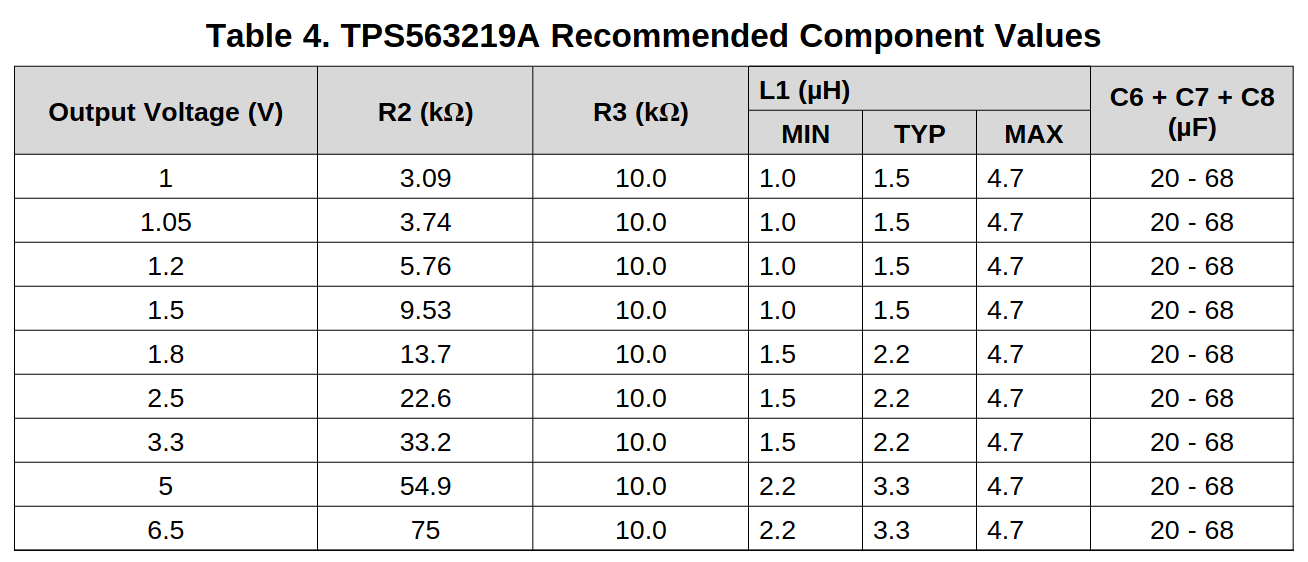
\includegraphics[width=0.8\textwidth]{conv-table.png}
    \caption{Tabela doboru komponentów z noty katalogowej \cite{st:buck}}
    \label{fig:conv-table}
\end{figure}

Projekt wzorowano na schemacie z noty katalogowej, który przedstawiono na rysunku \ref{fig:buck}.
Na podstawie tabeli dobrano następujące wartości komponentów:
\begin{itemize}
    \item C1: \SI{22}{\micro\farad} \SI{10}{\volt}
    \item C29: \SI{22}{\micro\farad} \SI{10}{\volt}
    \item L1: \SI{2.2}{\micro\henry} \SI{9.2}{\ampere} \SI{14.5}{\milli\ohm}
    \item R1: \SI{56}{\kilo\ohm}
    \item R2: \SI{10}{\kilo\ohm}
\end{itemize}

\begin{figure}[H]
    \centering
    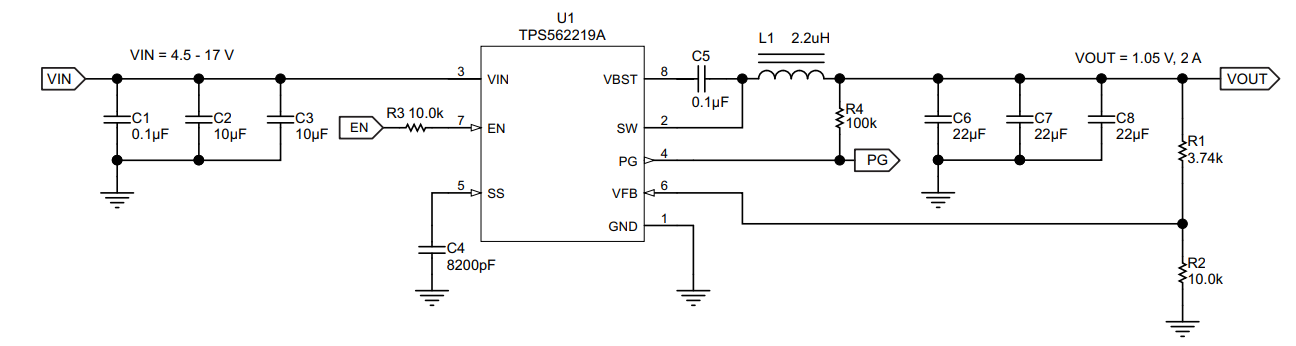
\includegraphics[width=1\textwidth]{buck.png}
    \caption{Typowe połączenie układu TPS563219ADDFR \cite{st:buck}}
    \label{fig:buck}
\end{figure}

Kondensator dołączony do wyprowadzenia SS (soft start) oraz kondensator dołączony do pinu VBST został skopiowany z układu z noty katalogowej, gdyż nie jest to krytyczny element i nie ma potrzeby doboru wartości pod 
kątem zastosowania w zegarze.

Zdecydowano się na użycie kondensatorów ceramicznych, gdyż są one mniejsze i mają lepszy ESR niż elektrolityczne, co ma znaczenie przy przetwornicach impulsowych,
gdzie mamy wyższe częstotliwości przełączania. Przy zbyt dużym ESR kondensatora może on się nagrzewać, co prowadzi do jego uszkodzenia.
Kondensatory ceramiczne natomiast cechują się tak małym ESR, że producent nie podaje tej wartości w notach katalogowych, gdyż jest ona zbyt mała, by miała znaczenie.

Cewkę dobrano, biorąc pod uwagę jej stosunek oporu do ceny. Zdecydowano się na cewkę o oporze \SI{14.5}{\milli\ohm}, 
gdyż jest to najniższa wartość, jaką udało się znaleźć w sklepach elektronicznych w sensownej cenie i dość małej obudowie.

Dodano również kondensator filtrujący \SI{100}{\nano\farad} na pinie VCC, aby zredukować szumy z linii zasilania.
Schemat elektryczny zaprojektowanego modułu przedstawiono na rysunku \ref{fig:buck-schemat}.

\begin{figure}[H]
    \centering
    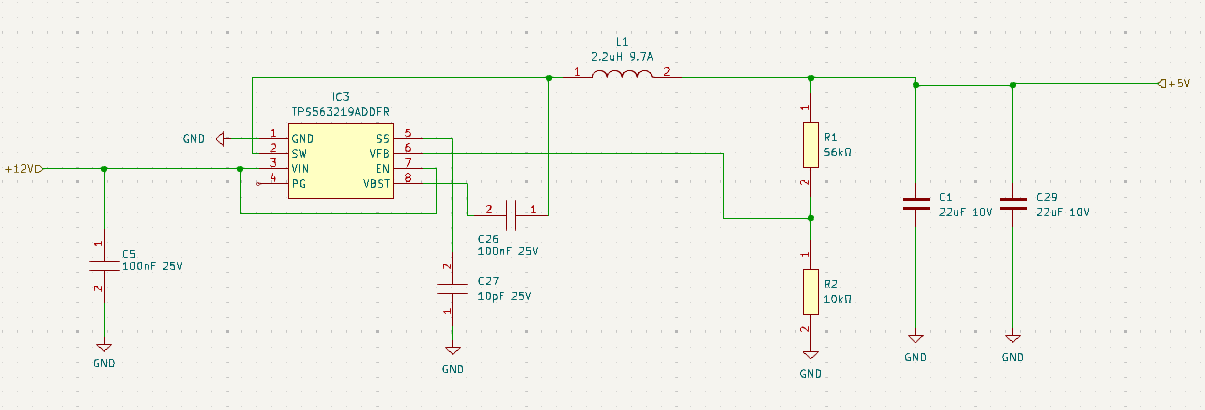
\includegraphics[width=1\textwidth]{5vTo12V_ schemat.png}
    \caption{Schemat elektryczny modułu przetwornicy z \SI{12}{\volt} na \SI{5}{\volt}}
    \label{fig:buck-schemat}
\end{figure}

\end{document}
